\section{Experiments}
\label{sec:experiment}
%\KZ{Give a little preamble here.}
In this section, we discuss some end-to-end experimental results 
comparing ChatMatch and some baseline methods. 
We also show some ablation studies with different settings of 
ChatMatch.

\subsection{Experiment Settings}

\subsubsection*{Description of Six Bots} 
We pick six chitchat chatbots to evaluate in our experiments:
\begin{itemize}
\item BB: Blender Bot \citep{roller2020recipes} which is a 
90M-parameter generative model following the training 
of \citet{shuster2020dialogue} and then finetuned on 
blended skill talk tasks \cite{smith2020together}.

\item CS: A Seq2Seq model with Control \citep{see2019makes} trained on ConvAI2 \citep{dinan2019second}. Here, we use the 
specificity-controlled WD model (with WD repetition control) 
provided in this paper.
\item CR: The response-relatedness WD model 
(with WD repetition control) provided in the paper about 
Controllable Seq2Seq \citep{see2019makes}
\item UG: A large pre-trained seq2seq Transformer finetuned on ConvAI2 
with vocab unlikelihood which sets parameter 
$\alpha =1e0$ \citep{li2020dont}
\item DG: DialoGPT medium \citep{zhang2020dialogpt} fine-tuned 
on ConvAI2. 
\item DD: Image Seq2Seq model trained on all DodecaDialogue tasks 
and fine-tuned on Convai2. \citep{shuster2020dialogue}
\end{itemize}
 
\subsubsection*{Baseline Evaluation Approaches}
We choose three automatic evaluation metrics and one human evaluation 
metric to compete with ChatMatch: 
\begin{itemize}
\item PPL: Perplexity \\
Perplexity (PPL) is a common metric for evaluating language models. 
Lower perplexity means that the generated sequence is 
the more likely to be close to a human sentence.
\item TA: Token Accuracy \\
Token Accuracy is used to measure the generation accuracy 
of each token, which refers to the ratio of the number of 
correctly predicted tokens to the total number of predicted tokens.
\item CC: Context Coherence \\
As language model usually predicts the next token according 
to previous tokens, Context Coherence captures the 
coherence between sentences naturally. We use this metric 
from ~\citet{pang-etal-2020-towards} to measure the coherence and 
consistency between the sentences generated by chatbots and the 
context.
\item STB: \textit{Spot The Bot}  \\
We also choose the recent proposed interactive manual evaluation metric \textit{Spot The Bot} \citep{deriu-etal-2020-spot} as our baseline. 
After collecting dialogues between chatbots and humans, 
we cut the dialogue logs into segments for every 2, 3, 5 exchanges, 
and distribute them to human judges. It is up to human judges to decide 
whether the chat is between humans, bots or unsure for each exchange. 
The scores for being recognised as human is larger than that as unsure and then as a bot. Finally, the dominant round will 
accumulate scores for the corresponding chatbot. 
We calculate the total score of each chatbot in the competition 
with all other chatbots and rank all chatbots according to the total scores.
\end{itemize}

%We also choose the recent proposed interactive manual evaluation metric  \textit{Spot The Bot} \citep{deriu-etal-2020-spot} as our baseline. In order to reproduce their evaluation %approach in a more simple way, we ask three college students who are skilled in English to be our annotators. We mix up our generated bot2bot chat logs with some human-bot %conversations and then cut them into short segments. Next, our annotators will give each turn a label which tells if the speaker is a bot from their prospectives. 


\subsubsection*{Ground Truth for Rankings}
 In order to obtain rankings that can be reliably used as ground truth, 
we asked 6 college students who are fluent in English to chat 
with each of the six bots and then manually assess the ability of 
the bots. Three dimensions (non-repetitiveness, consistency and 
diversity) are used to help them complete the ranking task 
which are rated on a 5-point Likert-scale. They can decide to 
stop the conversation whenever they feel confident enough to score
on these three dimensions. We set the maximum rounds of conversation 
to be 20. After finishing all the chats with six bots,  
the judges will provide their scores and overall rankings.

We use Kendall ranking correlation ($\tau$)  to evaluate the correlation 
among human judges. Their inter-agreement is shown at the last line of \tabref{tab:main}. In this paper, we use agreement to express correlation as well. We observe a good correlation among human judges. Later, we will compare the agreement between the evaluation metrics and human judges with their inter-agreement.  


\subsubsection*{Parameters settings for ChatMatch}

We describe the parameters settings for our framework
at different evaluation levels as follows: 
\begin{itemize}
\item  For each game, we choose the total number of rounds of the conversation to be 100 to ensure a sufficient process for distinguishing their abilities.
\item  Since the players of our tournament are chitchat bots used 
for daily conversations, the starting utterance is always set to
a daily routing sentence.
\item  At tournament evaluation level, we have 30 games (15 matches) 
in total for the whole tournament because each bot will play with
every other bot. We consider two approaches for scoring 
(macro and micro) as we describe in \secref{sec:approach}.
\end{itemize}


\subsubsection*{Experiment environment settings}
Our interactive chattings among the well-trained chatbots are running on a NVIDIA GeForce RTX 2080 machine with a 8GB RAM and 6 × Intel (R) Xeon (R) CPU E5-2678 v3 @ 2.50GHz.   
\begin{figure*}[th]
\centering
\includegraphics[width=0.7\textwidth]{macro.eps}
\caption{Scoreboard (Macro) and Rankings of 6-bot Tournament by ChatMatch.}
\label{fig:macro}
\end{figure*}

\subsection{Main Results }
\subsubsection*{ChatMatch Final results}
Here we use a common scoring table used in sports match to show our match results in \figref{fig:macro}. 
As we can see,  BB scores the top in our scoring framework (both for micro and macro). 
BB is a competitive bot as it aims at performing well in multiple chitchat test sets in different domains. 
CS and CR come in second and third respectively. They score quite close to each other as they use the same fine-tuned baseline seq2seq model, which only differ in the 
choice of specific parameters for some improvement in different aspects. 
DG and DD score close to each other. UG is always losing the match and ranks at the bottom. 
We can find an obvious difference between the scores of  
''the loser'' and the other five bots.

\subsubsection*{Final Scoring of Bots}

We show the native scores obtained by using different baseline evalution metrics and human rankings in \tabref{tab:baseline-scoring}. BB ranks the best with most of the metrics we have tested here (STB, Macro, Micro and Human Rankings). BB is considered to be the most competitive bot here, which is tranined on various tasks focusing on engagingness, knowledge and empathy. 
These evaluation results are consistent with the ground truth. DD ranks the best in two common automatic metrics PPL and TA while two controllable seq2seq models CR and CS rank the worst, which is inconsistent with our human evaluation results. 
PPL can only evaluate whether the sequence generated by the model is close to human language without considering the context. 
These evluation results are weakly correlated to human rankings. TA reflects whether the generated response matches the ground truth of the dataset. As reasonable responses are not limited to ground truth itself, it is difficult to correctly evaluate the ability of the chatbot with static scripts. In the process of calculating the CC metric, it tends to give a higher score to the shorter response, so BB and other chatbots that prefer to generate a longer sequence can not get a reasonable evaluation.
%\KZ{Need more explanations about why we got these automatic results.
%And compared to human, discuss a bit...}

\begin{table*}[ht!]
\centering
\small
\begin{tabular}{lrrrrrr}
%\hline
\toprule
& BB & CS & CR & UG & DG & DD  \\ \midrule
PPL & 11.31 & 22.86 &22.86 &11.42 & 12.39 & \textbf{11.19}  \\
TA & \textbf{0.47} & 0.39& 0.39 & \textbf{0.47} & 0.45& \textbf{0.47}  \\
CC& 0.47 & 0.61 & \textbf{0.72} &0.58  & 0.69 & 0.59  \\ 
STB & \textbf{1} & 2 & 6& 5 & 4 & 3\\
Macro  &\textbf{15}  &  12&9 & 0& 4& 4\\
Micro & \textbf{100}& -221 & -125 &  -876 & -761 & -609\\ 
Micro Rankings &\textbf{1} &3 &2 &6 &5 &4 \\ \midrule
Human Rankings & \textbf{1} & 4& 3& 5&6 & 2\\
\bottomrule
\end{tabular}
\caption{Native Scores by Competing Evaluation Methods and Human.}
\label{tab:baseline-scoring}
\end{table*}



\begin{table}[th!]
\centering
\small
\begin{tabular}{lccccc}
\toprule
 & Non Repeat & Consist &Diversity & Overall \\ \midrule
PPL & -  &- &- &0.12   \\
TA&-  &- &- &0.12 \\
CC&- &- &- &-0.06\\
STB &- &- &-&0.55 \\
Macro& 0.46& 0.10&-&0.50\\ 
Micro&\textbf{0.65} &\textbf{0.30}&-&\textbf{0.62} \\\midrule
Human & 0.57 &  0.30  &0.59 & 0.46\\ 
 \bottomrule
\end{tabular}
\caption{Agreement between all evaluation frameworks and 
human judges on Non repetitiveness, Consistency and 
overall performances (Kendall's $\tau$). }
\label{tab:main}
\end{table}

\tabref{tab:main} shows the final correlation results of the baseline models and our models. We put some dashes in the table as the baseline evaluation models are not able to provide specific tests about non repetitiveness and consistency. We can tell from the \tabref{tab:main} that common automatic evaluation metrics such as PPL, TA and CC present poor correlations 
with human judgements as their ranking agreement coefficient is close to zero, 
which indicates a weak agreement. \textit{Spot The Bot} correlates well with human judgements as they 
mainly depend on human annotations themselves.

The agreement for our macro and micro metrics are 0.50 and  0.62 respectively. Our best micro scoring metric performs well with $\tau = 0.62$ which is even better than the agreement among human judges ( $\tau = 0.46$ ). This indicates a good correlation between our models and human judgements. 

We also notice a good correlation between ChatMatch's micro scoring metric
and human judges on Non-repetitiveness dimension as 
well. However, neither of our two scores fare very well with
consistency, probably because it is harder for us to 
detect implicit inconsistencies using our rules while human can better pick up such inconsistencies.
\subsection{Ablation Studies}
We will only focus on our results with micro scoring approach 
from now onwards as it is generally better than macro scoring.

\subsubsection*{Effect of the start of the game}

As most of the chitchat bots we test in the competition 
were for open domain, we provide a list of contexts about 
everyday life as the candidates for the starting utterances, 
which involves greeting, declarative sentence and a question.  
Their performances and simple examples are shown 
in \tabref{tab:multi-context}.

\begin{table}[th!]
\centering
\small
\begin{tabular}{llr}
%\hline
\toprule
 & Example  & Avg ($\tau$)\\ \midrule
Greetings  & ``Hi! How are you?'' & 0.35  \\
Declarative  & ``I got a fever this morning.'' & 0.48  \\
Question  & ``Where are you from?'' & \textbf{ 0.62}  \\
Average  & & 0.35  \\
\bottomrule
\end{tabular}
\caption{
Agreement with human judgements using different starting utterances. 
Average denotes agreement after summing up scores with 
three different starts.}
\label{tab:multi-context}
\end{table}

 While looking at the final results shown as \tabref{tab:multi-context},
 We find that all of the three starting utterances lead to a 
good correlation with human. The model with a start as a question 
performs the best. We also sum the scores of three sentences to 
simulate a multi-game match.  However, comparing the multi-game 
match result with the results of a single starting sentence, 
we do not find a significant difference. That's because when two 
bots are free to talk without human intervention, they prefer 
to steer the chat to their ``comfort zones'' (e.g., talking about 
their basic personal information) rather than stick to the ball 
``started'' by ChatMatch. 

\subsubsection*{Different number of exchanges in a game} 

We also test ChatMatch with different number of exchanges in a game. 
The results shown in \figref{fig:exchanges} indicate that the 
longer we let the chatbots chat with each other, more likely our framework can rank them correctly. We finally decide to let them 
expose their flaws by engaging them in 100 exchanges 
of conversation which is enough to get good results. 

\begin{figure}[th]
\centering
	\includegraphics[width=\columnwidth]{exchanges.eps}
\caption{Kendall's $\tau$ with different number of exchanges.}
\label{fig:exchanges}
\end{figure}

\subsubsection*{Similarity functions} 
In our experiment, we provide a set of simple similarity functions 
to detect repetition and inconsistency in chat logs which are: 
tf-idf cosine similarity, mean of Word2Vec sentence cosine similarity 
and Bag-of-Word Jaccard coefficient. While comparing the final correlation 
results of these three similarity functions, we find that 
the three different similarity functions perform almost the same. 
We then compare their running time and we find that the system
using tf-idf as similarity function is the most time efficient 
one as we don't need to calculate similarity between two turns at 
each time step. The results are shown in \tabref{tab:similarity}.

\begin{table}
\small
\centering
\begin{tabular}{lcccc}
\toprule
&tf-idf & Word2Vec & Jaccard \\ \midrule
Agreement & 0.62 &  0.62 & 0.62\\
Time &\textbf{ 1 min 6 secs} &  2 min & 1 min 56 secs\\ \bottomrule
\end{tabular}
\caption{Comparison of three similarity functions. Agreement is calculated by Kendall's $\tau$.}
%\KZ{Run a few times to get average timem then update the number in time efficiency section.}
\label{tab:similarity}
\end{table}  

\subsubsection*{Stand-alone tests of Non-Repetitiveness, 
Consistency and Memory}
Additionally, we compare the effect of each individual 
scoring component(Non-Repetitiveness, Consistency, 
and Ability to Memorize) 
at game level by setting the two other coefficients to zero. 
As \tabref{tab:coef} shows, the model that only scores for 
Non-repetitiveness and Memory ability presents significant 
correlation to human results. The scoring of Consistency 
performs worse as our simple rules can only capture some instances
of inconsistency. This kind of inconsistency are always common 
in less capable bots. More potent inconsistency 
detection rules will be introduced in the future.

\begin{table}
\small
\centering
\begin{tabular}{lcccc}
\toprule
& Non-repeat & Consist & Memory \\ \midrule
Micro & 0.57  & 0.35    & \textbf{0.59} \\ \bottomrule
\end{tabular}
\caption{Agreements with human ($\tau$) on stand-alone tests.}
\label{tab:coef}
\end{table}

\subsubsection*{Choices for three coefficients: 
repeat($r$), inconsistency($c$) and bonus($b$)}

Here we test two sets of coefficients introduced in \ssecref{ssec:scoring}: 
\begin{itemize}
\item Identical weight choices $r = c = b = 1$
\item Fine-tuned weights: we fine-tune three coefficients with a linear regression model according to the rates about three dimensions and the overall rankings provided by human judges, we set $r = 0.37, c = 0.64, b = -0.02$.
\end{itemize}

 The final results with these two sets of coefficients are: $\tau_i = 0.62, \tau_f = 0.46 $ respectively. As identical weight choices with $r=c=b=1$ performs better, we decide to keep using the identical weight set in other part of our experiments.  
 

\subsection{Time Efficiency}

As for timing, a human judge takes more than 30 minutes on average to complete 
the conversations with all 6 bots, decide ratings on three dimensions and then rank the bots. 
Our system only requires about 1 min 6 secs on average to 
complete a game, 
which is an 100-exchange conversation. As all 30 games can be processed in 
parallel, the total time cost for evaluating all the 6 bots is less than
2 minutes. To put it in perspective, when we evaluate the same
6 bots by \textit{Spot The Bot} framework, it takes on average one hour for
each human judge to complete the ranking.


\subsection{Discussion}
In our experiments, we only test chatbots used for daily chatting. 
It would also be useful to test chatbots from other domains 
(e.g., domain-specific bots with specialized knowledge, 
empathetic bots used for entertainment, etc.) in the future.
The rules that we have used at the moment are still very simple. 
In order to detect more subtle weakness in bots, we probably 
need a more comprehensive setup for future design of the system . 

